
%(BEGIN_QUESTION)
% Copyright 2011, Tony R. Kuphaldt, released under the Creative Commons Attribution License (v 1.0)
% This means you may do almost anything with this work of mine, so long as you give me proper credit

Try to interpret this Manchester-encoded digital signal as viewed on an oscilloscope display, and explain why the task is difficult (or impossible) without further information:

$$\includegraphics[width=15.5cm]{i02415x01.eps}$$

\vfil 

\underbar{file i02415}
\eject
%(END_QUESTION)





%(BEGIN_ANSWER)

This is a graded question -- no answers or hints given!

%(END_ANSWER)





%(BEGIN_NOTES)

Since all cycles of this waveform have the same period, we cannot tell by looking at it whether it is a repeated sequence of identical bits (e.g. 00000000, 11111111) or an alternating sequence of bits (e.g. 01010101).  What we need is to see another cycle with a different period.  If this different period is shorter (i.e. a reversal), then we know the rising and falling edges shown are a sequence of alternating 1's and 0's.  If the different period is longer, then we know every other edge shown in this waveform is a reversal, which makes the data stream either a sequence of 0's or a sequence of 1's, depending on where this sequence starts in relation to the longer pulse.

\vskip 10pt

Even if we happened to know the clock period for this particular waveform, we might still be helpless to properly interpret it.  If we knew that the frequency of this waveform matched the clock frequency, then we would know all of the transitions were ``real'' bits, and that this waveform represented an alternating string of 1's and 0's (i.e. {\tt 101010101010}.  However, if the waveform's frequency happened to be twice that of the known clock frequency, all we would know is that every other transition was a reversal, but we still wouldn't know which of them were reversals and which were ``real'' bits.  In other words, it could be a series of repeating 1's ({\tt 111111}) or it could be a series of 0's ({\tt 000000}).

%INDEX% Electronics review: Manchester encoding

%(END_NOTES)


